\documentclass[catalan, a4paper]{scrartcl}

% encoding
\usepackage[utf8]{inputenc}
\usepackage[T1]{fontenc}
\usepackage{lmodern}
\usepackage{babel}

% formatting and fixes
\frenchspacing
\usepackage[style=spanish]{csquotes}
\MakeAutoQuote{«}{»}
\usepackage{subcaption}

% general design preferences (page, paragraph indent/space, margins, class options, ...)
\setlength{\parskip}{10pt}
\setlength{\parindent}{0pt}
%\pagestyle{plain}

% ADD ANY SPECIFIC PACKAGES HERE
% (CHEMISTRY, CODE, PUBLISHING)
\usepackage{siunitx}
\usepackage{tikz}
\usepackage{commath}
\usepackage{mathtools}
\usepackage{nicefrac}
\usepackage{minted}

% other options

%\usemintedstyle{xcode}
\setminted{
  %frame=leftline,
  %framesep=12pt,
  xleftmargin=15pt,
  breaklines,
  breakautoindent,
  breakindent=1em,
}

% hyperlink setup / metadata
\usepackage{hyperref}
\AfterPreamble{\hypersetup{
  pdftitle={Memòria P2B — PSAVC QP2019},
  pdfsubject={DAT},
}}

\newcommand{\haskellfunc}[1]{\texorpdfstring{\mintinline{haskell}{#1}}{#1}}

% document metadata
\author{Alba Mendez}
\title{Memòria pràctica 2B\\
{\small DAT QT2019}}
\date{8 de novembre de 2019}

\begin{document}

%\begin{minipage}{\columnwidth}
\maketitle
%\end{minipage}


\part{Introducció}

En aquesta segona part de la pràctica es preten consolidar coneixements més
avançats de Haskell vists a teoria. Per fer-ho, es dona una aplicació web
CGI feta en Haskell, que implementa una calculadora de números complexos.
Es demana que l'estudiant completi alguns mètodes d'un dels mòduls.

També es dona un entorn de desenvolupament amb un script que compila i desplega
l'aplicació, però m'he construit un en el meu portàtil per poder treballar
en local. A banda d'alguns errors (en les noves versions de Haskell, \mintinline{haskell}|Monoid|
és una subclasse de \mintinline{haskell}|Semigroup|) no hi ha hagut problemes
significatius.

\clearpage

\part{Estructura de l'aplicació}

\begin{figure}
\centering
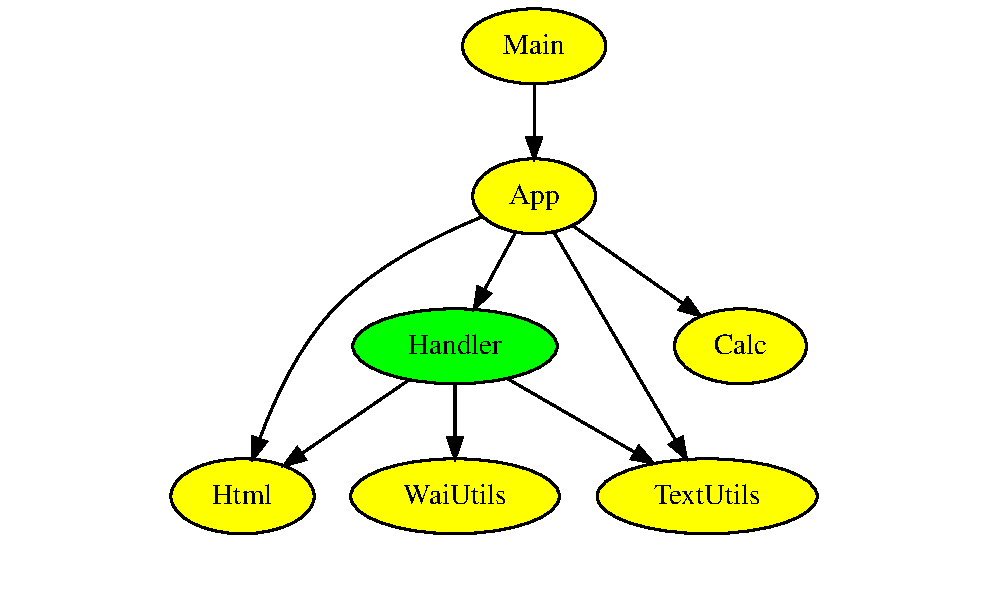
\includegraphics[width=\columnwidth]{deps.pdf}
\caption{\label{fig:deps} Els mòduls de l'aplicació i les dependències entre ells.}
\end{figure}

Començarem comentant breument cadascun dels mòduls que conformen l'aplicació.
El graf de dependències es pot veure a la figura~\ref{fig:deps}, donada pel professor.

\section{Mòduls d'utilitat}

Primer presentarem aquells mòduls que no tenen rellevància específica
a aquesta aplicació, i només serveixen per fer el codi més elegant o
implementen accions molt genèriques.

\paragraph{TextUtils} Aquest mòdul simplement conté implementacions de funcions
típiques de conversió de/a text (\mintinline{haskell}|show|, \mintinline{haskell}|read|,
\mintinline{haskell}|readEither| i \mintinline{haskell}{showsPrec}), però
que accepten (o retornen) \mintinline{haskell}{Text} en comptes de \mintinline{haskell}{String}.
S'han anomenat respectivament \mintinline{haskell}|showt|, \mintinline{haskell}|readt|,
\mintinline{haskell}|readtEither| i \mintinline{haskell}{showtPrec}.

\paragraph{Html} Aquest mòdul és molt simple i preten simplificar la generació d'HTML.
Es defineix un writer monad, \mintinline{haskell}{HtmlM a},
i unes funcions que generen nodes HTML típics fent servir aquest monad, com
ara el \emph{doctype}, un element (amb els seus atributs), o text (escapat apropiadament).

\paragraph{WaiUtils} Aquí s'implementen operacions típiques amb WAI:

\begin{itemize}
  \item Obtenir els paràmetres de la petició.
  \item Descodificar les dades de la sessió (una llista de parells clau-valor textuals) a
        partir del contingut de la \emph{cookie} corresponent, i fer la operació inversa.
  \item Generar una resposta HTTP sencera a partir del contingut HTML donat (text).
  \item Generar una resposta HTTP que redirigeixi a la URL donada.
  \item Generar una resposta HTTP d'error, amb el codi i missatges donats.
\end{itemize}

\section{Mòduls d'aplicació}

\paragraph{Main} En primer lloc tenim aquest mòdul, que és el punt d'entrada
de l'executable CGI. El seu codi és molt senzill, només defineix \mintinline{haskell}{main}:

\begin{minted}{haskell}
main :: IO ()
main = do
    -- try :: Exception e => IO a -> IO (Either e a)
    r <- try $
        -- CGI adapter: run :: Application -> IO ()
        run calcApp
    case r of
        Right _ -> pure ()
        Left exc -> do
            -- Exception on initialization
            putStrLn "Status: 500 Internal Server Error"
            putStrLn "Content-Type: text/plain"
            putStrLn ""
            putStrLn "Exception on initialization (while excution of 'calcApp'): "
            putStrLn $ "    " ++ show (exc :: SomeException)  
\end{minted}

Veiem que s'executa \mintinline{haskell}{calcApp} mitjançant
el mètode \mintinline{haskell}{run} de \mintinline{haskell}{Network.Wai.Handler.CGI}.
En cas que hi hagi qualsevol error en l'execució, s'imprimeix una resposta
500 manualment, que conté la descripció de l'excepció.

\paragraph{App} La funció \mintinline{haskell}{calcApp} es defineix al mòdul \textbf{App},
que dona pas a la lògica principal de l'aplicació. Es defineixen i implementen
les possibles operacions que es poden fer amb els nombres, es renderitza la
pàgina HTML i es gestionen les accions que faci l'usuari.

Per aconseguir-ho, aquest codi fa servir principalment \textbf{Html} i els dos mòduls
que s'expliquen a continuació, \textbf{Calc} i \textbf{Handler}.

\paragraph{Calc} Aquest mòdul implementa la gestió de l'estat de la
calculadora:

\begin{itemize}
\item Es defineix \mintinline{haskell}|CalcStack|, que
representa l'estat de la calculadora (una pila de valors).
\item Es defineix \mintinline{haskell}|CalcInstr|, que representa
una operació amb aquest estat: ja sigui una manipulació simple
de la pila (com afegir, treure o intercanviar valors) o una operació
unària o binària genèrica amb els valors de dalt de la pila.
\item Es defineix \mintinline{haskell}|solveCalc|, que aplica una operació de dalt (o serie d'operacions) a un estat concret, retornant el nou estat.
\end{itemize}

Cal indicar que aquest mòdul és genèric i no tracta directament amb
nombres complexos. La pila pot contenir valors de qualsevol tipus,
i no s'implementa cap operació unària o binaria concreta.

\paragraph{Handler} Aquest és el mòdul que l'estudiant ha de completar.
Es defineix un monad \mintinline{haskell}|Handler a|, que té les següents propietats:

\begin{itemize}
\item State monad: Manté un estat que es va passant entre acció i acció.
Aquest estat emmagatzema principalment les dades de sessió (una llista de parells clau-valor, com
s'explica a dalt).
\item Reader monad: Permet operar amb la petició HTTP quan encara no la tenim.
\item A més, encapsula una acció I/O que retorna el resultat de tipus \mintinline{haskell}|a|,
i el nou estat.
\end{itemize}

Es tracta doncs d'un mòdul genèric que construeix una capa d'abstracció
sobre la funcionalitat de \mintinline{haskell}|WaiUtils|, per fer encara més senzilla
la gestió de les dades de la sessió i dels paràmetres de la petició.

En la secció següent s'entra en detall sobre aquest mòdul i la implementació
de les funcions demanades.

\clearpage

\part{Solució de la pràctica}

A continuació s'explicarà l'estructura del mòdul en més detall,
i s'exposaran les solucions a les funcions que es demana implementar.

\section{Implementació del monad}

En primer lloc es defineix el monad com hem explicat en la secció
anterior. Se'ns demana implementar \mintinline{haskell}|pure| (àlias
de \mintinline{haskell}|return|) i la funció \emph{bind} del monad.

\vskip 1em

Anem a la funció \mintinline{haskell}|pure|. Per definició, agafa un
valor \mintinline{haskell}{x} i l'encapsula dins el monad. La implementació
és fàcil, només cal cridar el constructor (\mintinline{haskell}|HandlerC|)
passant una lambda que, donada una petició i un estat, retorna una acció
I/O pura de \mintinline{haskell}{x} i aquest estat:

\begin{minted}{haskell}
pure x = HandlerC $ \ _ st0 -> pure ( x, st0 )
\end{minted}

La funció \emph{bind} és una mica més complicada. Es crida el constructor
amb una lambda com abans, però ara cal passar la petició i l'estat al primer
monad, per obtenir una acció I/O. El resultat d'\emph{aquesta} acció I/O
es passa a \mintinline{haskell}|f| per obtenir un nou monad. Llavors cal
cridar \mintinline{haskell}|runHandler| i passar-li la petició i el nou estat,
per obtenir l'acció I/O final:

\begin{minted}{haskell}
HandlerC hx >>= f = HandlerC $ \ req st0 -> do
    ( x, st1 ) <- hx req st0
    (runHandler $ f x) req st1
\end{minted}

A continuació s'implementen funcions que fan servir el monad anterior per
manipular les dades de la sessió, i també una per obtenir el mètode de la petició,
que és la que implementarem a continuació.

\section{Funció \haskellfunc{getMethod}}

La funció es defineix com \mintinline{haskell}|getMethod :: Handler Method|.
Com el seu nom indica, simplement retorna el mètode de la petició. Per
implementar-la primer busquem com extreure el mètode de la petició, i veiem
que es fa amb la funció de WAI \mintinline{haskell}|requestMethod|.

Llavors només cal construir un monad amb aquest resultat, però no podem fer
servir \mintinline{haskell}|pure| perquè la petició està encapsulada en el
monad. De tota forma, la implementació és molt similar a \mintinline{haskell}|pure|:

\begin{minted}{haskell}
getMethod = HandlerC $ \ req st0 ->
    pure ( requestMethod req, st0 )
\end{minted}

\section{Funcions \haskellfunc{getSession\_} i \haskellfunc{setSession\_}}

Finalment es demana implementar \mintinline{haskell}|getSession| i \mintinline{haskell}|setSession|,
que donada una clau, emmagatzemen o retornen el valor que té associat en l'estat
de la sessió:

\begin{minted}{haskell}
getSession :: Read a => Text -> Handler (Maybe a)
setSession :: Show a => Text -> a -> Handler ()
\end{minted}

Abans però, implementarem \mintinline{haskell}|getSession_| i \mintinline{haskell}|setSession_|.
Aquestes son les versions «base» que accepten i retornen el valor en text,
mentre que les versions sense \mintinline{text}|_| fan servir \mintinline{haskell}|showt|
o \mintinline{haskell}|readt| per convertir el valor a text primer:

\begin{minted}{haskell}
getSession_ :: Text -> Handler (Maybe Text)
setSession_ :: Text -> Text -> Handler ()    
\end{minted}

\vskip 1em

Comencem amb \mintinline{haskell}|getSession_|. La seva implementació
és molt similar a la de \mintinline{haskell}|getMethod|, però aquí farem
servir \mintinline{haskell}{hsSession} per extreure les dades de sessió de l'estat,
i després la funció estàndard \mintinline{haskell}{lookup} per extreure el valor
correponent a la clau donada:

\begin{minted}{haskell}
getSession_ name = HandlerC $ \ req st0 ->
    pure ( lookup name $ hsSession st0, st0 )
\end{minted}

Anem amb \mintinline{haskell}|setSession_|. Aquesta funció ens ve ja mig
implementada; s'extreu la sessió de l'estat com hem fet abans i es reemplaça
el valor en la clau donada:

\begin{minted}{haskell}
setSession_ name value = HandlerC $ \ req st0 -> do
    let newsession = (name, value) : filter ((name /=) . fst) (hsSession st0)
    error "Handler.setSession_: A completar per l'estudiant"
\end{minted}

L'únic que queda, doncs, és reemplaçar la sessió per \mintinline{haskell}|newsession|
i retornar el nou estat. Això ho podem fer amb la funció \mintinline{haskell}|hsSetSession|.
Per tant, el resultat és:

\begin{minted}{haskell}
setSession_ name value = HandlerC $ \ req st0 -> do
    let newsession = (name, value) : filter ((name /=) . fst) (hsSession st0)
    pure ( (), hsSetSession newsession st0 )
\end{minted}

\section{Funcions \haskellfunc{getSession} i \haskellfunc{setSession}}

Ara és fàcil implementar \mintinline{haskell}|getSession| i \mintinline{haskell}|setSession|
fent servir aquestes funcions. La segona és fàcil, només cal cridar \mintinline{haskell}|setSession_|
amb el valor convertit:

\begin{minted}{haskell}
setSession name value = setSession_ name (showt value)
\end{minted}

\mintinline{haskell}|getSession| és una mica més complex ja que \mintinline{haskell}|getSession_ name|
retorna el resultat dins el monad; cal mapejar-lo. Però el monad no conté
directament \mintinline{haskell}|Text| sinó \mintinline{haskell}|Maybe Text|;
per tant no podem mapejar el valor amb \mintinline{haskell}|readt|, ho hem de fer amb \mintinline{haskell}{(>>= readt)}:

\begin{minted}{haskell}
getSession name = (>>= readt) <$> getSession_ name
\end{minted}

\end{document}
